\section{Related Work}
\label{sec:formatting}


\subsection{Numerical}

Currently, multi-channel thresholding is a popular method to distinguish smoke pixels from pixels containing dust, clouds or other phenomenon with similar signatures \cite{threshold}. Thresholds are determined by using historical, labeled data to extract optimal radiance values for each channel that corresponds with the labeled class. These methods are tuned to particular biogeographies and often have issues with generalization to new locations with varying fuel types \cite{thresh_geog}.

\subsection{Analyst} 
In contrast to the numerical thresholding approach, human visual inspection of satellite imagery is another commonly used method for smoke identification. Trained analyst inspect satellite imagery and label the smoke by hand. An example of hand-labeled annotations is the National Oceanic and Atmospheric Administration (NOAA) Hazard Mapping System (HMS) fire and smoke product \cite{hms, hms_val}. For the HMS smoke product, trained satellite analysts use movement characteristics to help identify smoke by scanning through a time series of satellite imagery. When visual inspection indicates smoke, the analyst will draw a polygon that corresponds to the geolocation and density of smoke. By design of the product, the HMS annotations have varying time resolution and are released on a rolling but undefined schedule ranging from one to multiple times a day as observation conditions permit. If expanded beyond the current North American boundary, this method will not be as scalable as an automated approach and is limited by the availability of analysts and their time. 

NOAA manages environmental satellite programs such as the HMS program, an operational system that uses an aggregation of satellite data to generate active fire and smoke data. To train our model, we implement a supervised learning framework that uses the HMS analyst smoke product as truth labels during the model training process.

HMS smoke analysis data gives the coordinates of the smoke perimeter as a polygon and classifies the smoke by density within a given time window. The time windows can range from instantaneous (same start/end time) to lengths of 22 hours. While the true bounds of the smoke can change within the larger time spans, the analyst is making an approximation that should reflect the smoke coverage over the duration of the time window. The density information is qualitatively determined by each analyst based on the apparent smoke opacity in the satellite imagery and categorized as either light, medium or heavy as seen in figure \ref{densities}a \cite{hms_web}.

\subsection{Deep Learning}

To address the challenges associated with thresholding and manual labels, we can look towards innovative approaches and recent technological advancements in computer vision. Machine learning methods have shown potential in improving the accuracy and efficiency of satellite-based wildfire smoke detection and monitoring. For instance, SmokeNet, uses a convolutional neural network (CNN) based framework to determine if a scene of MODIS satellite imagery contains smoke \cite{smokenet}. Another study, that looked at a singular wildfire event, also used a CNN to identify smoke on a pixel-wise basis using imagery from Himiwari-8 \cite{larsen}. Additionally, Wen et al. developed a CNN architecture that takes GOES-East imagery as input and the HMS-generated annotations for the target labels during training \cite{smoke_goes}. 

The success of deep learning methods, such as CNNs, relies heavily on the availability of a large, representative dataset \cite{data_size}. As laid out in table \ref{studies}, prior studies use relatively small numbers of samples, from 47 \cite{wang} to 6825 \cite{smoke_goes}, where one sample represents a satellite image with a singular time and geolocation. In contrast, benchmark datasets for image classification contain tens of thousands (CIFAR-10 \cite{cifar} and MNIST \cite{mnist}) to millions (CIFAR-100 and ImageNet \cite{imgnet}) of data samples. Keeping in mind the correlation between both the quality and quantity of data with model performance, we introduce the largest known smoke dataset, SmokeViz, containing over 180,000 samples.

\begin{table*}[h]
    \caption{Comparison of different studies including method used, dataset size, satellite source, number of channels used and if classification is performed at a pixel or image level.}\label{studies}
    \centering
    \begin{tabular}{ccccrrcrc}
        \toprule
        Reference & Method & \verb|#| Samples & Satellite & \verb|#| Channels & Level\\
        \midrule
        \cite{smokenet}& CNN & 6255 & MODIS & 5 & image\\
        \cite{smoke_goes}& CNN & 6825 & GOES-East & 5 & pixel\\
        \cite{larsen} & CNN & 975 & Himiwari-8 & 7 & pixel\\
        \cite{wang}& U-Net & 47 & Landsat-8 & 13 & pixel\\
        SmokeViz  & U-Net & 183,672 & GOES-East/West & 3 & pixel\\
        \bottomrule
    \end{tabular}
\end{table*}

Semi-supervised learning is an approach that can be used to increase the number of labeled samples in a dataset. This is done by leveraging a labeled dataset to generate new labels for an often larger, but unlabeled, dataset. Pseudo-labeling, a form of semi-supervised learning, uses labeled data to train an initial model, then runs that model on unlabeled data to predict pseudo-labels, and finally trains a new model using the pseudo-labels \cite{pseudo}. Since we do not know of any studies that have used this technique in this way, we introduce a variation of pseudo-labeling, not to increase the size, but to increase the quality of our dataset by generating pseudo-labels to select the best satellite image out of a given time-window to represent each smoke plume annotation.

\begin{figure*}
    \centering
    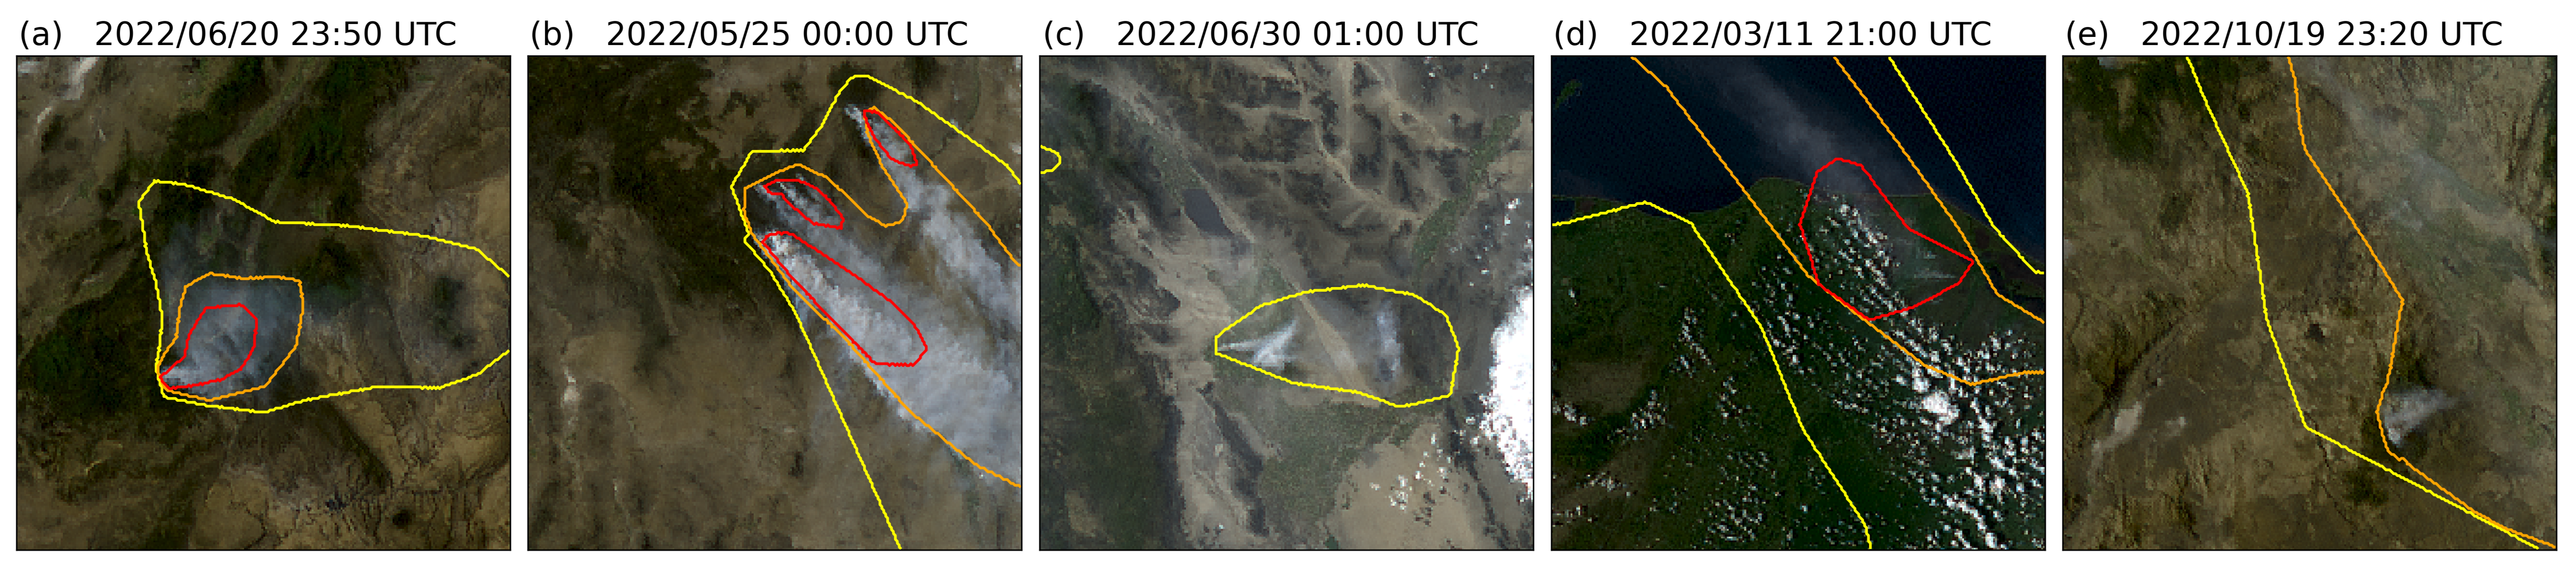
\includegraphics[width=\linewidth]{figures/variations2.png}
    \caption{HMS smoke annotations overlaid on GOES imagery, the yellow, orange and red contours indicate the extent of light, medium and heavy density smoke. (a) and (b) show a canonical examples of a smoke plumes. (c)-(e) show observable variations in the density labels.}\label{densities}
\end{figure*}

